The most popular type of wearable in 2019 is the smartwatch \cite{best_watches}. 
Smartwatches are devices worn on one's wrist,
equipped with sensors, and in some cases wireless communication capability for syncing data to a smartphone.
Some common examples of smartwatches are the Apple Watch (Figure \ref{fig:sub1}), 
Fitbit Charge (Figure \ref{fig:sub2}), and the Garmin Forerunner (Figure \ref{fig:sub3}),
all shown below in Figure \ref{watches:pictures}.
These devices are priced quite differently, carry different levels of functionality, and are
targeted towards different segments of the population. Shown below in Table \ref{watch:price} are 
prices for the watches listed above \cite{apple_price} \cite{fitbit_price} \cite{garmin_price}.

\begin{figure}[h]
    \centering
    \begin{subfigure}{.5\textwidth}
      \centering
      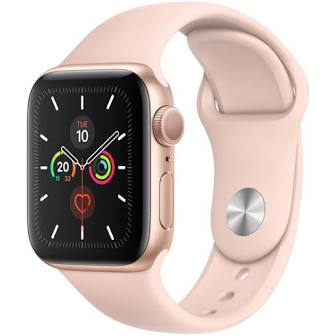
\includegraphics[width=.4\linewidth]{media/apple_pic.jpeg}
      \caption{Apple Watch Series 5 \cite{apple_price}}
      \label{fig:sub1}
    \end{subfigure}%
    \begin{subfigure}{.5\textwidth}
      \centering
      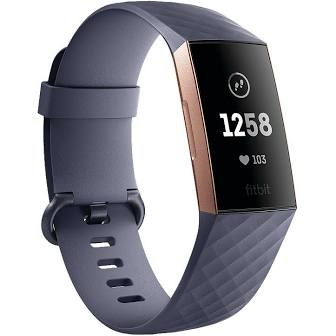
\includegraphics[width=.4\linewidth]{media/fitbit_pic.jpeg}
      \caption{Fitbit Charge 3 \cite{fitbit_price}}
      \label{fig:sub2}
    \end{subfigure}
    \begin{subfigure}{.5\textwidth}
        \centering
        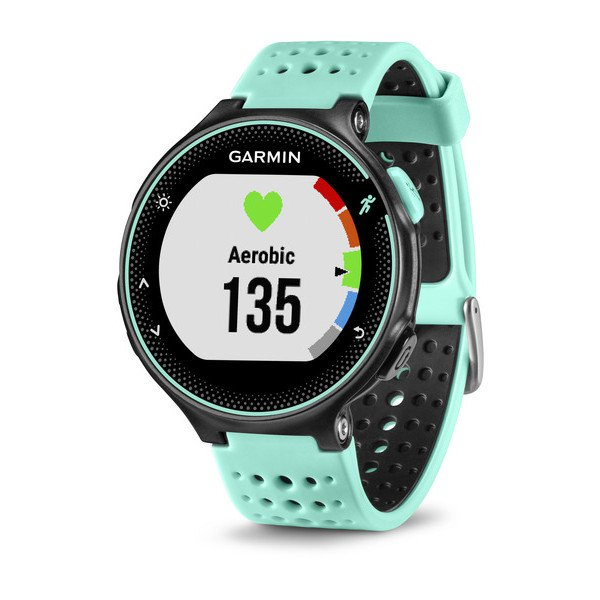
\includegraphics[width=.4\linewidth]{media/garmin_pic.jpeg}
        \caption{Garmin Forerunner 235 \cite{garmin_price}}
        \label{fig:sub3}
      \end{subfigure}
    \caption{Smartwatches discussed in this report.}
    \label{watches:pictures}
\end{figure}


\begin{table}[h]
    \centering
    \caption{Smartwatch Prices}
    \csvautotabular{data/prices.csv} 
    \label{watch:price} 
\end{table}






